\begin{problem} {Search and Heuristics}

\begin{center} 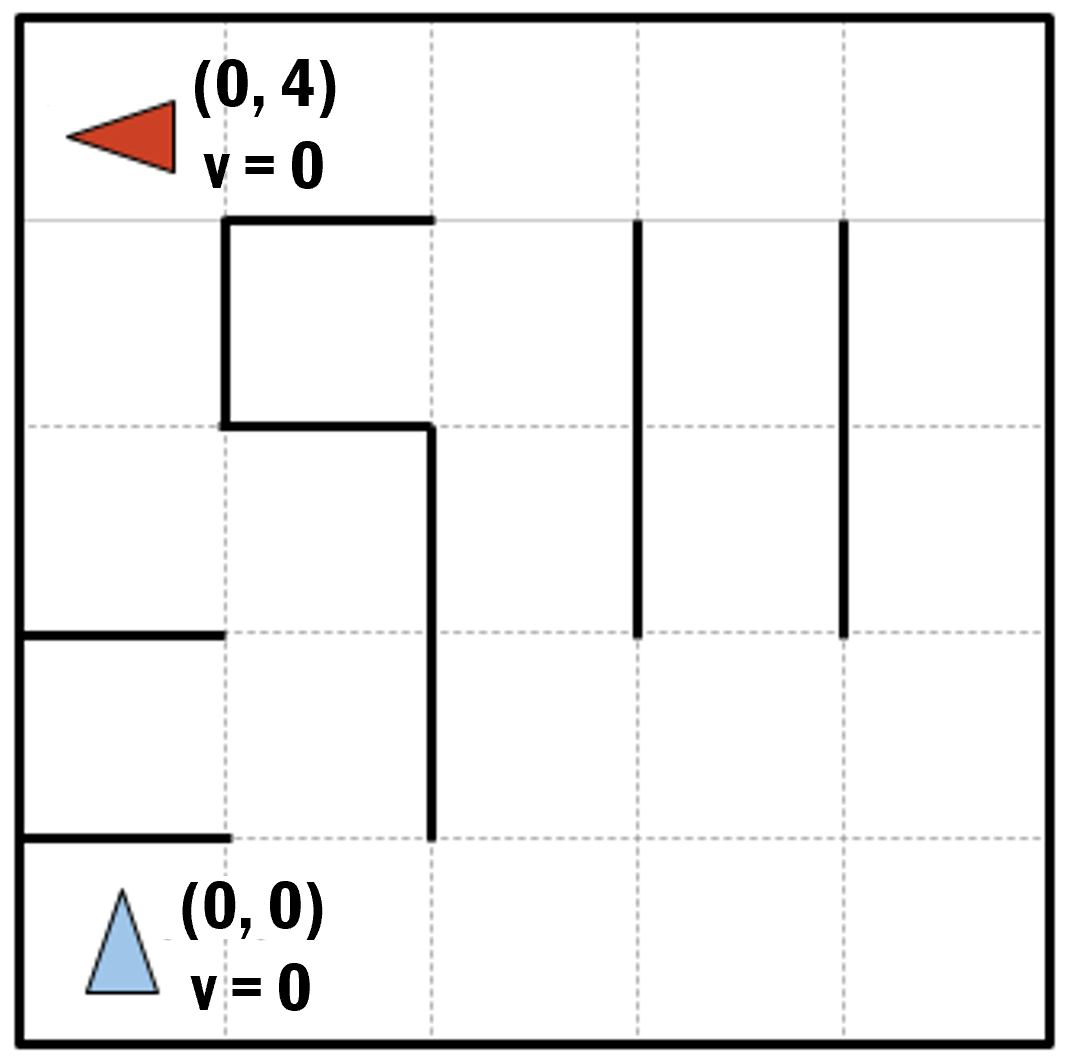
\includegraphics[scale=.33]{figures/movingagent.png} 
\end{center}

Imagine a car-like agent wishes to exit a maze like the one shown above. The agent is directional and at all times faces some direction $d \in (N, S, E, W)$. With a single action, the agent can \textit{either} move forward at an adjustable velocity $v$ or turn.

The moving actions are \textit{faster}, \textit{maintain} and \textit{slower}. For these actions, the agent then moves a number of squares equal to its \textbf{new} adjusted velocity. Let $v$ denote the agent's current velocity and let $v'$ denote the agent's new adjusted velocity.
\begin{itemize}[noitemsep,topsep=0pt]
    \item \textit{Faster}: $v'$ = $v$ + 1
    \item \textit{Slower}: $v'$ = $v$ - 1
    \item \textit{Maintain}: $v'$ = $v$
\end{itemize}

The turning actions are \textit{left} and \textit{right}, which change the agent’s direction by 90 degrees. Turning is only permitted when the velocity is zero (and leaves it at zero). 
\begin{itemize}[noitemsep,topsep=0pt]
    \item \textit{Left}: change the agent’s direction by 90 degrees counterclockwise
    \item \textit{Right}: change the agent’s direction by 90 degrees clockwise
\end{itemize}

For example, if the agent is currently on (0, 0) facing north with velocity 0 (as pictured) and wants to get to (2, 0) facing east with velocity 0, the sequence of actions will be: \textit{right, faster, maintain, slower}.

Illegal actions include
\begin{itemize}[noitemsep,topsep=0pt]
    \item Any action that would result in a collision with a wall
    \item Any action that would reduce $v$ below 0 or above a maximum speed $V_{max}$ 
    \item Maintaining a velocity of 0
\end{itemize}

The agent’s goal is to find a plan which parks it (stationary) in the goal direction on the exit square using as few actions (time steps) as possible. Note that the cost of a path is defined by the number of actions the agent takes.

\begin{question}[2] Suppose the agent wants to take the leftmost path (i.e., the one that passes through (1,2)) from the start (0,0) facing north to the goal (0,4) facing west. Write down the sequence of actions for it to take.

\solutionspace{2cm}{15cm}{Actions:}{\Onea}

\end{question}

\newpage

\begin{question}[2]
If the grid is M by N, what is the size of the state space? You should assume that all configurations are reachable from the start state.

\solutionspace{2cm}{10cm}{State Space Size:}{\Oneb}

\end{question}

\begin{question}[4] 
What is the maximum branching factor of this problem?
Draw an example state (x, y, orientation, velocity, grid/walls) that has this branching factor, and list the set of available actions. For example, in the above picture, if the agent was in (0, 0) facing North with a velocity of 0, the branching factor would be 2. The agent could either turn left or right.

You may assume that illegal actions are simply not returned by the problem model and therefore not counted in the branching factor. You do not necessarily have to use the example grid above. Make sure to label your drawing.

\solutionspace{1.5cm}{10cm}{Maximum Branching Factor:}{\Onecmax}

\solutionspace{5cm}{15cm}{Maximum Branching Example State and Available Actions:}{\Onecmaxexample}

\end{question}
 
\begin{question}[4]
Is the Manhattan distance from the agent’s location to the exit’s location admissible?

If not, draw an example state (x, y, orientation, velocity, grid/walls) where this heuristic overestimates at that state, and specify: 1) the heuristic value at that state and 2) the actual cost from that state to the goal.

You may assume that illegal actions are simply not returned by the problem model. You do not necessarily have to use the example grid above. Make sure to label your drawing, including the goal state.

\hspace{5mm}
\solution{\emptycircle}{\OnedYes} Yes
\hspace{5mm}
\solution{\emptycircle}{\OnedNo} No

\solutionspace{6cm}{15cm}{Example State, Heuristic Value, Actual Cost: }{\Onedreason}

\end{question}

\newpage
 
\begin{question}[4]
Is the following heuristic admissible? \textit{Manhattan distance / $V_{max}$}.

If not, draw an example state (x, y, orientation, velocity, grid/walls) where this heuristic overestimates at that state, and specify: 1) the heuristic value at that state and 2) the actual cost from that state to the goal.

You may assume that illegal actions are simply not returned by the problem model. You do not necessarily have to use the example grid above. Make sure to label your drawing, including the goal state.

\hspace{5mm}
\solution{\emptycircle}{\OneeYes} Yes
\hspace{5mm}
\solution{\emptycircle}{\OneeNo} No

\solutionspace{6cm}{15cm}{Example State, Heuristic Value, Actual Cost:}{\Oneereason }
\end{question}

\begin{question}[2]
If we used an inadmissible heuristic in A* search, could it change the completeness of the search? 

\hspace{5mm}
\solution{\emptycircle}{\OnefYes} Yes
\hspace{5mm}
\solution{\emptycircle}{\OnefNo} No

\solution{}{\OneFReason}
\end{question}

\begin{question}[2]
If we used an inadmissible heuristic in A* search, could it change the optimality of the search? 

\hspace{5mm}
\solution{\emptycircle}{\OnegYes} Yes
\hspace{5mm}
\solution{\emptycircle}{\OnegNo} No

\solution{}{\OneGReason}
\end{question}

\begin{question}[2]
Give a general advantage that an inadmissible heuristic might have over an admissible one.

\solutionspace{3.5cm}{15cm}{Answer:}{\Oneh}
\end{question}

\end{problem}

